\documentclass{beamer}
\usepackage{ctex, hyperref}
\usepackage[T1]{fontenc}

% other packages
\usepackage{latexsym,amsmath,xcolor,multicol,booktabs,calligra}
\usepackage{graphicx,pstricks,listings,stackengine}

\author{苏星午\quad 闫溥扬\quad 王廷轩}
\title{生产运作管理报告}
\subtitle{}
\institute{}
\date{\today}
\usepackage{Tsinghua}

\usefonttheme[onlymath]{serif}
\setbeamercolor{normal text}{fg=black!35}
\setbeamercolor{alerted text}{fg=black}

% defs
\def\cmd#1{\texttt{\color{red}\footnotesize $\backslash$#1}}
\def\env#1{\texttt{\color{blue}\footnotesize #1}}
\definecolor{deepblue}{rgb}{0,0,0.5}
\definecolor{deepred}{rgb}{0.6,0,0}
\definecolor{deepgreen}{rgb}{0,0.5,0}
\definecolor{halfgray}{gray}{0.55}

\lstset{
    basicstyle=\ttfamily\small,
    keywordstyle=\bfseries\color{deepblue},
    emphstyle=\ttfamily\color{deepred},    % Custom highlighting style
    stringstyle=\color{deepgreen},
    numbers=left,
    numberstyle=\small\color{halfgray},
    rulesepcolor=\color{red!20!green!20!blue!20},
    frame=shadowbox,
}


\begin{document}

\kaishu
\begin{frame}
    \titlepage
    \begin{figure}[htpb]
        \begin{center}
            
\includegraphics[width=0.2\linewidth]{pic/Tsinghua_University_Logo.png}
        \end{center}
    \end{figure}
\end{frame}

\begin{frame}
    \tableofcontents[sectionstyle=show,subsectionstyle=show/shaded/hide,subsubsectionstyle=show/shaded/hide]
\end{frame}


\section{引入}

\begin{frame}{LLM推理服务}
    \begin{itemize}[<+-| alert@+>] % 当然，除了alert，手动在里面插 \pause 也行
        \item LLM处理一次请求分两个阶段
            \begin{itemize}
                \item Prefill阶段，和
                \item Decode阶段
            \end{itemize}
        \item 其中Prefill阶段处理用户输入的 prompt，建立 KV cache；
        \item Decode阶段则一个 token 一个 token 地生成回答。
        \item 现行 Batch processing 同时处理多个请求
        \item 调度器要决定：每一次 GPU forward pass 里，到底放哪些请求、哪些 token、多少 prefill、多少 decode。
    \end{itemize}
\end{frame}

\section{LLM Inference Setup}
\begin{frame}{Iteration}
    \begin{itemize}[<+-| alert@+>] 
        \item 一个请求可以表示为 $(x_1, x_2, ..., x_p, x_{p+1}, ..., x_{p+d})$
        \item 一次iteration指一次模型 forward pass
        \item 每一次 iteration，调度器可以从多个请求中挑 token，组成一个 batch，一起送进 GPU
    \end{itemize}
\end{frame}

\begin{frame}{Batch \& Token Load}
    \begin{itemize}[<+-| alert@+>] 
        \item 用 $B$ 代表一个batch，它包含了若干请求中的全部或部分token
        \item 用 $b$ 代表该 batch 中的 token 总数
        \begin{itemize}
            \item $b\le b_{max}$，token budget.
        \end{itemize}
    \end{itemize}
\end{frame}

\begin{frame}{Batch Processing Time}
    \begin{itemize}[<+-| alert@+>] 
        \item 实验观察到，在现实负载下，只要 token load $b$ 固定，batch 里面具体是哪些请求、prefill 和 decode 怎么混合，对处理时间影响相对较小。
        \item 对token load 为 $b$ 的batch，处理时间 $t_b$ 建模为 $t_b = c + a\lceil \frac{b}{b_0}\rceil$
        \begin{itemize}
            \item $b_0:$ 硬件或系统中的 token block 大小
        \end{itemize}
    \end{itemize}
\end{frame}

\section{Basic LLM Queueing Model}
\begin{frame}{Basic LLM Queueing Model}
    \begin{itemize}[<+-| alert@+>] 
        \item 离散时间。时间被划分为离散的时刻 $n\in \{1,2,3,...\}$ 
        \item 到达请求 $i$ 有两个长度
        \begin{itemize}
            \item $v_p(i): $ prefill token数
            \item $v_d(i): $ decode token数
            \item $(v_p(i),v_d(i))$ 独立同分布
        \end{itemize}
        \item 定义 $m_p:=\mathbb{E}[v_p(i)],\quad m_d:=\mathbb{E}[v_d(i)]$ 
        \item 每个时刻 $n$ 到达的请求数记为 $a_n$ ，独立同分布
            \begin{itemize}
                \item 定义平均到达率 $\lambda :=\mathbb{E}[a_n]$ 
            \end{itemize}
        \item 每个时刻带来的平均工作量是 $\lambda (m_p+m_d)$ 
    \end{itemize}
\end{frame}

\begin{frame}{Basic LLM Queueing Model}
    \begin{itemize}[<+-| alert@+>] 
        \item 在时刻 $n$ 定义系统中没有完成的请求集合为 $\mathcal{Q}_n$
        \item 对每个未完成的请求 $i\in \mathcal{Q}_n$，定义
            \begin{itemize}
                \item $P_i(n)$ ：剩余的prefill token数
                \item $D_i(n)$ ：剩余的decode token数
            \end{itemize}
        \item 当前batch的剩余处理时间记为 $R(n)$ 
        \item 系统状态记为 $X(n)=\left( R(n),\{(P_i(n),Q_i(n)):i\in \mathcal{Q}_n\}\right)$ 
        \begin{itemize}
            \item 构成离散时间马尔可夫链
        \end{itemize}
    \end{itemize}
\end{frame}

\begin{frame}{The Main Conclusion}
    若系统负载满足
    \[
    \lambda(m_p + m_d) > b_{\text{max}} / t_{b_{\text{max}}},
    \]
    则在任何调度算法下，未处理的token总数都会发散：
    \[
    \mathbb{P}\left\{ \lim_{n \to \infty} |X(n)| = \infty \right\} = 1,
    \]

    其中 \( |X(n)| = \sum_{i \in \mathbb{Q}_n} (P_i(n) + D_i(n)) \).
\end{frame}


\section{LLM Queuing & Token Length and Batch Size}

\begin{frame}{Two stages of LLM Reasoning}
    \begin{itemize}
        \item LLM推理请求分为两个阶段：\textbf{prefill} 和 \textbf{decode}
        \item \textbf{Prefill}：一次性全输入，并发性高。batch提高会显著提升吞吐。\emph{受输入的token数量影响。}
        \item \textbf{Decode}：逐个生成输出token，并发性低（只能串行）。\emph{受输出的token数量影响。在输出较长的情况下，占据总推理时间的大部分。}
    \end{itemize}
\end{frame}

\begin{frame}{Padding问题}
    \begin{itemize}
        \item Transformer模型要求一个batch内所有序列长度完全相同，因而需要有padding补齐的环节。
        \item 在decode阶段，传统的dynamic batching会导致短输出被迫等待长输出。
        \item Batch大提高吞吐，但是padding拖慢响应速度。
    \end{itemize}
\end{frame}


\section{排队论分析：Max-Limit Clipping}

\begin{frame}{M/G/1 队列建模}
    \begin{itemize}
        \item 考虑没有Batch的情况，队列建模为 \textbf{M/G/1}
        \begin{itemize}
            \item \textbf{M}：请求到达服从Poisson过程。
            \item \textbf{G}：输出token长度决定了推理过程（即服务时间）的时长，且token输出数比较随机，故认为其服从一般分布。
            \item \textbf{1}：只考虑一台服务器。
        \end{itemize}
        \item 服务时间 $S$ 的建模：推理时间与输出token数呈线性关系
        \begin{equation*}
            S = a \cdot n + c
        \end{equation*}
        此处 $n$ 表示输出token数。
    \end{itemize}
\end{frame}

\begin{frame}{平均等待时间与 Max-Token 限制}
    \begin{itemize}
        \item 由上述表达式，可以求得等待时间 $E[W]$ 与 $n_{\max}$ 的关系。经过手动模拟后画成图如下：
    \end{itemize}
    \vfill
    \begin{figure}
        \centering
        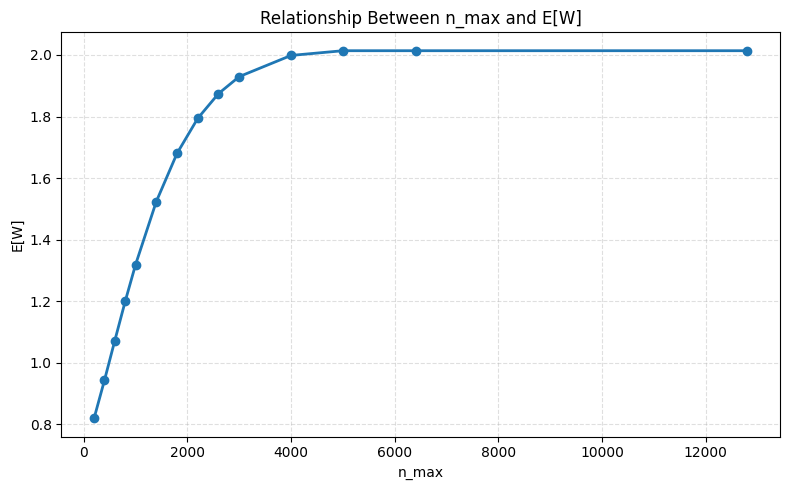
\includegraphics[width=0.7\linewidth]{pic/slide4_img11_图片_19.png}
        \caption{$E[W]$ 与 $n_{\max}$ 的关系图}
    \end{figure}
    \vfill
    \begin{itemize}
        \item \textbf{结论：}输出token长度影响LLM推理延迟；添加max-token限制，可在牺牲生成质量（较小）的代价下提高响应速度。
    \end{itemize}
\end{frame}


\section{Dynamic Batching 的影响}

\begin{frame}{传统 Dynamic Batching}
    \begin{itemize}
        \item 服务时间同时取决于batch大小 $b$，和batch内最大输出token长度 $l$
        \item Prefill阶段和Decode阶段分别处理：
        \begin{itemize}
            \item Prefill阶段：同时处理多个请求的输入部分
            \item Decode阶段：逐token生成
        \end{itemize}
        \item 可以计算出平均等待时间上界 $E(W)$：
    \end{itemize}
    \vfill
    \begin{figure}
        \centering
        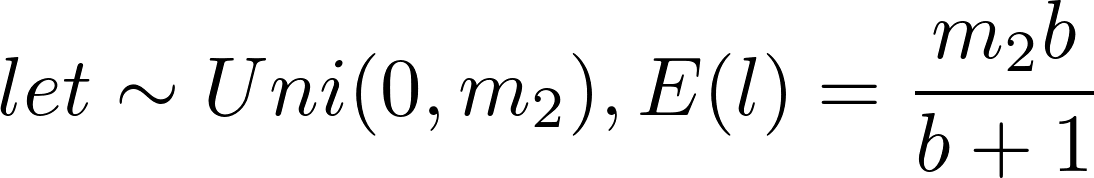
\includegraphics[width=0.35\linewidth]{pic/slide5_shape5_sub0_334E55B0-647D-440b-865C-3EC943EB4CBC-12.png}
        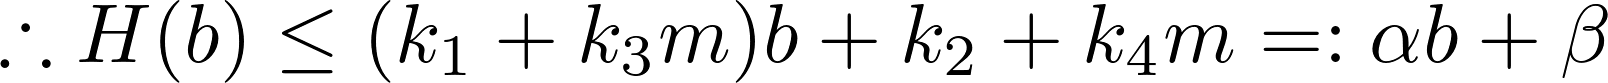
\includegraphics[width=0.35\linewidth]{pic/slide5_shape5_sub1_334E55B0-647D-440b-865C-3EC943EB4CBC-13.png}
    \end{figure}
\end{frame}

\begin{frame}{E(l) 与拖尾分布的影响}
    \begin{figure}
        \centering
        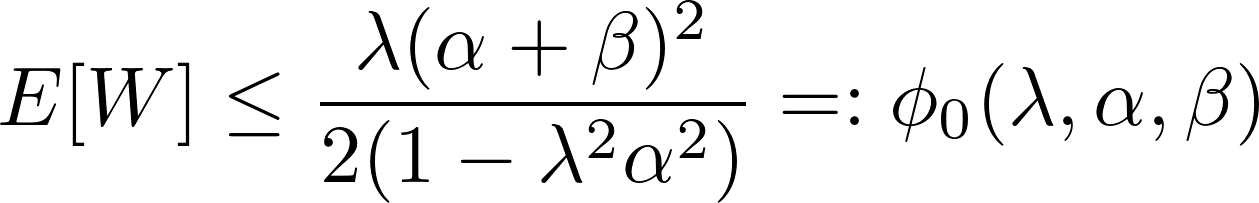
\includegraphics[width=0.7\linewidth]{pic/slide6_img3_334E55B0-647D-440b-865C-3EC943EB4CBC-11.png}
    \end{figure}
    \begin{itemize}
        \item $E(l)$ 随 $b$ 增大而增大，但增长速度逐渐变慢
        \item 在\textbf{轻尾分布}下，Dynamic Batching 无批大小上限效果很好
        \item 在\textbf{重尾分布}下，无限制 Dynamic Batching 会因为偶尔出现的极长输出导致严重 Padding 浪费，延迟恶化
    \end{itemize}
\end{frame}

\begin{frame}{Fixed Batching}
    \begin{itemize}
        \item \textbf{M/D$_b$/1} 队列：积累达到 $b$ 个请求才开始服务，且服务时间不随批内请求特征变化
        \item \textbf{轻尾分布}中：批大小 $b$ 越大，推理速度 $\mu[b]$ 越高
        \item \textbf{重尾分布}中：存在最优批大小 $b^*$。超过 $b^*$ 后，$\mu[b]$ 开始下降（Padding浪费）
    \end{itemize}
    \begin{figure}
        \centering
        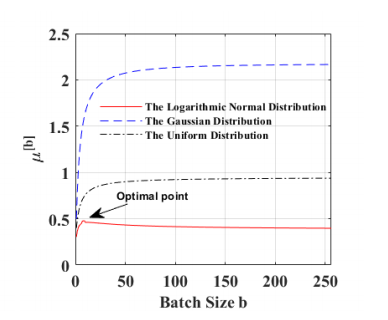
\includegraphics[width=0.6\linewidth]{pic/slide7_img5_图片_5.png}
    \end{figure}
\end{frame}

\begin{frame}{Elastic Batching}
    \begin{itemize}
        \item 每生成一个token就检查哪些已完成，完成的返还并移除出batch
        \item 新的批处理时间：
    \end{itemize}
    \begin{figure}
        \centering
        
\includegraphics[width=0.5\linewidth]{pic/slide8_shape4_sub1_334E55B0-647D-440b-865C-3EC943EB4CBC-18.png}
    \end{figure}
    \begin{itemize}
        \item 其中，$n_b$：批内最长的输出token数量；$E(N)$：单个请求输出token数期望值
        \item 在\textbf{重尾分布}下，优于Dynamic Batching和Fixed Batching
        \item \textbf{结论：}在batching场景下，elastic batching的排队延迟最低；dynamic batching和fixed batching则需要结合输出token分布来选择参数。
    \end{itemize}
\end{frame}


\section{总结}

\begin{frame}{Key Takeaways}
    \begin{itemize}
        \item 输出token长度影响LLM推理延迟，且\textbf{长尾分布}会显著拉高平均响应时间
        \item 添加max-token限制，可在牺牲生成质量的代价下提高响应速度
        \item 在 batching 场景下，elastic batching 的排队延迟最低
        \item Dynamic batching 和 fixed batching 则需要结合输出token分布来选择参数
    \end{itemize}
\end{frame}


\end{document}